\DiaryEntry{Permutations, 3 (Number of Fixed Points)}{2016-01-04}{Combinatorics}

Consider a set of $n$ elements: In total there are $n!$ permutations - How many permutations are there with $k$ fixed points? This number is callled \href{https://en.wikipedia.org/wiki/Rencontres_numbers}{Recontres Number} and will be denoted as $D_{n,k}$.

For example, chose $n=5$ and consider the permutation

\[
\sigma=\begin{pmatrix}
1 & 2 & 3 & 4 & 5 \\
2 & 5 & 3 & 1 & 4
\end{pmatrix}
\]

We have one fixed point: $\sigma(3) = 3$.

In order for a permutation to have \textbf{one} fixed point, any of the $n$ elements can become the fixed point. The other $n-1$ must not have a fixed point, therefore they must form a derangement. There are $!(n-1)$ such derangements. Therefore, the number of permutations with exactly one fixed point is

\bee
D_{n,1} = n !(n-1)
\eee

In a similar way we can argue for the number of permutations having two fixed points: There are $n \choose 2$ ways to select the two fixed points and the other $n-2$ elements must form a derangement.
Therefore, we have

\bee
D_{n,2} = {n \choose 2} !(n-2)
\eee

Generalizing, we obtain

\be\label{2016-01-04:eq1}
D_{n,k} = {n \choose k} !(n-k)
\ee

for the number of permutations of $n$ elements having $k$ fixed points.

\subsubsection{Some Values}

can be found \href{https://en.wikipedia.org/wiki/Rencontres_numbers}{here} and are shown below.

\begin{figure}
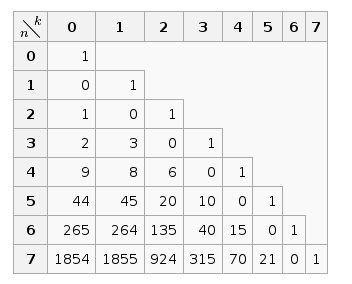
\includegraphics{images/recontres_numbers.png}
\end{figure}

The following properties can be observed:

\begin{itemize}
\item  It can be seen that $D_{n,n-1} = 0$; there are no permutations of $n$ elements having $n-1$ fixed points; the last element must also be a fixed point.
\item  There is one $n$-permutation with $n$ fixed points: $D_{n,n} = 1$ which is the identity permutation.
\item  The number of permutations without a fixed point (i.e. $k=0$) equals the number of derangements; i.e. $D_{n,0} = !n$.
\item  The row-sum equals the number of permutations; i.e. $\sum_{k} D_{n,k} = n!$. We can split the permutations into groups having the same number of fixed points. Summing over the group-sizes yields the total number of permutations.
\end{itemize}

\subsubsection{Probability of $k$ fixed points}

Now let's calculate the probability $P_{n,k}$ that a randomly chosen permutation has $k$ fixed points. The number of permutations having $k$ fixed points is given by \eqref{2016-01-04:eq1}; in order to get the probability we divide this by the number of all permutations (having length $n$) which is $n!$. We therefore have

\bee
P_{n,k} = {n \choose k} \frac{!(n-k)}{n!}
\eee

Inserting the definition of ${n \choose k} = \frac{n!}{(n-k)! k!}$ and obtain

\be\label{2016-01-04:eq2}
P_{n,k} = \frac{n!}{(n-k)! k!} \frac{!(n-k)}{n!} = \frac{!(n-k)}{(n-k)! k!} = \frac{1}{k!} \frac{!(n-k)}{(n-k)!}
\ee

Let's consider this in the case of large $n$; from the previous entry \ref{2015-12-26:entry} we know that $\lim_{n \rightarrow \infty} \frac{!n}{n!} = e^{-1}$ and therefore

\be\label{2016-01-04:eq2}
\lim_{n \rightarrow \infty} P_{n,k} = \frac{1}{e k!}
\ee

As a cross-check, the probabilities must sum up to one; indeed we have $\sum_{k=0}^\infty \frac{1}{e k!} = \frac{1}{e} \sum_{k=0}^\infty \frac{1}{k!} = \frac{e}{e} = 1$ \qed.

Simulating things in Julia we can compare between \eqref{2016-01-04:eq1} and \eqref{2016-01-04:eq2}; for a fixed value of $n$ the difference becomes bigger for larger values of $k$. For $k=n-1$, the approximation yields a non-zero value (but from above we know that there are no permutations of $n$ elements having $n-1$ fixed points). For example, $n = 10, k=7$, the true value is $7.3 \cdot 10^{-5}$ and the approximation yields $6.6 \cdot 10^{-5}$. At $n = 10, k=10$, the true value is $10^{-7}$ whereas the approximation yields $2.7 \cdot 10^{-7}$, a much larger error. At $n=20$, the errors are much smaller, there is only a significant error for $k=20$. \qed

We can also calculate the expected number of fixed points in a randomly chosen permutation in the limit of large $n$; we have

\bee
\sum_{k=0}^\infty k \left( \lim_{n \rightarrow \infty} P_{n,k} \right) = \sum_{k=0}^\infty k \frac{1}{e k!} = \frac{1}{e} \sum_{k=0}^\infty k \frac{1}{k!} = \frac{1}{e} \sum_{k=0}^\infty \frac{1}{(k-1)!} = \frac{1}{e} e = 1
\eee

So in the limit of large $n$, we have an expected number of one fixed point in a randomly chosen permutation. \todo{can we calc the epxected value exactely, $\sum_{k=0}^n k \frac{1}{k!} \frac{!(n-k)}{(n-k)!}$? Numerically, the difference is extremely small...}


%%% Local Variables:
%%% mode: latex
%%% TeX-master: "journal"
%%% End:
